In this section I describe scoring rules that can be used to assess the performance of probabilistic forecasting models. The scoring rule framework allows us to define useful generalisations of well-known information quantities, such as entropy, mutual information and divergence. Based on this, scoring rules allow for defining rich geometries of probabilistic models, which can be exploited in a variety of statistical applications, such as parameter estimation, approximate inference and optimal experiment design.

Imagine we want to have build a probabilistic forecaster that predicts the value of a random quantity $\X$. We can describe any such probabilistic forecaster as a probability distribution $P(x)$ over the space of possible outcomes $\Xe$. After observing the outcome $X=x$ we want to assess how good our predictions were: \emph{scoring rule} is a general term to describe any function that quantifies this: if the outcome is $X=x$, and our prediction was $P$ we incur a score $\score (x,P)$. Scoring rules, by convention, are interpreted as losses, so lower values are better. A good example of scoring rules is the logarithmic score, or simply the log score: $\score_{\mbox{log}}(x,P) = -\log P(\x)$, which is used in maximum likelihood estimation. It is certainly a very important scoring rule and has several unique features (see section \ref{sec:logscore}), but it is not the only one. I will give further examples of scoring rules in section \ref{}. Mathematically, a scoring rule is any measurable function that maps an outcome-probability distribution pair onto real numbers: $\score:\Xe\times\probmeasures{\Xe}\mapsto\mathcal{R}\cup\{\infty\}$.

\section{Information quantities}

A scoring rule allows us to define the following, useful information quantities \cite[see also][]{Blaetal2332}.

\begin{definition}[Generalised entropy]
Given a scoring rule $\score:\Xe\times\probmeasures{\Xe}\mapsto\Reals$, let us define the generalised entropy of a distribution $P\in\probmeasures{\Xe}$ as follows:
\begin{equation}
	\genentropy{S}{P}= \expect{x\sim P} \score(x,P)
\end{equation}
\end{definition}


This entropy measures how hard it is to forecast the outcome on average, when true distribution $P$ of outcomes is known and used as the forecasting model. We can often think of this quantity as a measure of uncertainty in the distribution, and as we will see this quantity is also closely related to the Bayes-risk of decision problems (section \ref{sec:loss_scoring}).

A further quantity of interest is the divergence between two distributions $P$ and $Q$.

\begin{definition}[Generalised divergence]
Given a scoring rule $\score:\Xe\times\probmeasures{\Xe}\mapsto\Reals$, let us define the divergence between two distributions $P,Q\in\probmeasures{\Xe}$ as follows:
	\begin{equation}
		\divergence{\score}{P}{Q} = \expect{x\sim P} \score(x,Q) - \expect{x\sim P} \score(x,P)\mbox{.}\label{eqn:def_divergence}
	\end{equation}
\end{definition}

\TODO{Mention Bregman divergences \citep{http://bit.ly/Ojhpw4}}.

The divergence measures how much worse we are at forecasting a quantity $\X$ sampled from a distribution $P$ when instead of using the true distribution $P$, we use an alternative probability distribution, $Q$. Ideally, we would like to see that using the true model $P$ should always be better or at least as good as using any alternative model $Q$, but this is not automatically true for all scoring rules. A scoring rule that has this property is called a \emph{proper scoring rule}.

\begin{definition}[Proper scoring rule]
	$\score:\Xe\times\probmeasures{\Xe}\mapsto\Reals$ is a \emph{proper scoring rule} with respect to a class of distributions $\Qe$ if $\forall P,Q\in\Qe$ the following inequality holds:
	\begin{equation}
		\expect{x\sim P} \score(x,Q) \geq \expect{x\sim P} \score(x,P),
	\end{equation}
	or equivalently in terms of the divergence $\divergence{\score}{\cdot}{\cdot}$:
	\begin{equation}
		\divergence{\score}{P}{Q} \geq 0.
	\end{equation}
	
	The scoring rule $s$ is said to be \emph{strictly proper} w.\,r.\,t.\ $\Qe$ if equality holds only when $P=Q$.
\end{definition}

The divergence is a measure of the difference between two distributions $P$ and $Q$. Even if the scoring rule is proper, and therefore $\divergence{s}{P}{Q} \geq 0$ always holds, the divergence is normally non-symmetric, that is $\divergence{\score}{P}{Q} \neq \divergence{\score}{Q}{P}$. Divergences are often used to match or approximate some \emph{true} or \emph{ideal} distribution with something \emph{approximate}, so that the divergence between the truth and the approximation is minimal. As we can measure divergence in both ways, there is a question of which direction of divergence is to be calculated.

The divergence defined in \eqref{eqn:def_divergence} is a special case of Bregman divergences:

\begin{definition}[Bregman divergence]
	Let $H$ be a differentiable, strictly concave function on a convex domain $\Theta$. For $P,Q\in\Theta$ 
	\begin{align}
		\divergence{Bregman,H}{P}{Q} = H(P) - H(Q) + \scalar{\nabla H(Q)}{Q-P}
	\end{align}
\end{definition}


\begin{statement}[Generalised divergences $d_{\score}$ for strictly proper $\score$ are Bregman divergences]
	Let $S$ be a strictly proper scoring rule, with generalised entropy $\genentropy{\score}{P}$. If $\genentropy{\score}{P}$ is differentiable with respect to $P$, then the generalised divergence $\divergence{\score}{P}{Q} = \expect{x\sim P}\score(x,Q) - \genentropy{\score}{P}$ is a Bregman divergence with $H(\cdot) = \genentropy{\score}{\cdot}$.
\begin{proof}
	Review the definition of the entropy $\genentropy{\score}{P}$:
		\begin{equation}
			\genentropy{S}{P} = \expect{x \sim P}S(x,P) = \scalar{P}{S(\cdot,P)}
		\end{equation}
		Using this notation
		\begin{align}
			\nabla\genentropy{S}{P} &=  \nabla\scalar{P}{S(\cdot,P)}\\
				&= S(\cdot,P) + \scalar{P}{\nabla S(\cdot,P)}
		\end{align}
	The second term $\scalar{P}{\nabla S(\cdot,P)}=0$ because of strictly proper property of $S$. Thus
 		\begin{align}
 		 	\divergence{Bregman,\mathbb{H}_{S}}{P}{Q}&= \genentropy{S}{Q}  + \scalar{\nabla \genentropy{S}{Q}}{P-Q} -  \genentropy{S}{P} \\
 		 		&= \genentropy{S}{Q} + \scalar{S(\cdot,Q)}{P - Q} -  \genentropy{S}{P}\\
 		 		&= \scalar{S(\cdot,Q)}{P} - \genentropy{S}{P}\\
 		 		&= \divergence{S}{P}{Q}
 		\end{align}
 		Concavity of $\genentropy{\score}{P}$ also follows from strictly proper property $\divergence{S}{P}{Q}>0,P\neq Q$.
\end{proof}
\end{statement}

\begin{figure}
\begin{center}
	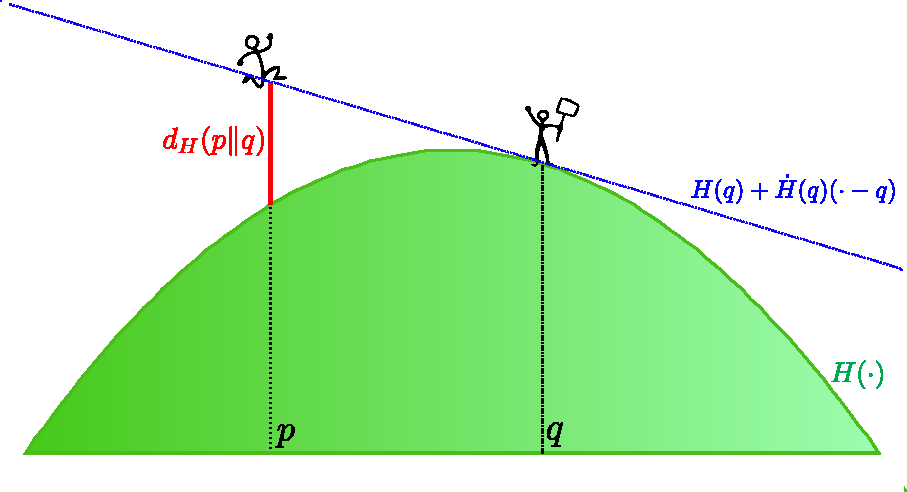
\includegraphics[width=0.8\columnwidth]{figs/embeddings/Bregman}
\end{center}
\caption{Pictorial illustration of Bregman divergences. Peter and Quentin are points who live on a convex hill, whose surface is described by the concave function $H(p)$. Peter lives at $(Q,H(P))$, Quentin at $(Q,H(Q))$. Because the hill is convex and they are both points, they cannot normally see each other, unless $P=Q$. Anyone above the tangential line $H[Q] + \dot{H}(Q)(\cdot-Q)$ can see Quentin, but Peter is normally below this line. If Peter wants to see Quentin, he has to jump up. The Bregman divergence $\divergence{H}{P}{Q}$ measures how high Peter has to jump to see Quentin. In this example $H$ was chosen to be the Brier (quadratic) entropy, so here the divergence is symmetric, but this is not generally the case.}
\end{figure}

An intuitive explanation of Bregman divergences is given in Figure \ref{fig:Bregman}.

\citep{Amari2010,Dawid2007}
Definition \eqref{eqn:def_divergence} suggests that the the first argument, $P$, should take the role of the true distribution, and $Q$ the approximate. \TODO{elaborate on this.}

So far we have only introduced quantities describing a single random variable, and comparing probability distributions over the same variable. We can extend the scoring rule framework to define information quantities that describe the relationship between multiple variables. A particularly useful quantity is the value of information, that measures the dependence between.

\begin{definition}[Generalised value of information]
	Let $X,Y$ be random variables with joint distribution $P\in\probmeasures{\Xe\times\Ye}$. Let $\score:\Xe\times\probmeasures{\Xe}\mapsto\Reals$ be a scoring rule over the variable $X$. We define the value of information in variable $Y$ about variable $X$ with respect to the scoring rule $\score$ as
	\begin{equation}
		\information{S}{X}{Y} =  \expect{x\sim P_{X}}\score(x,P_{X})- \expect{y\sim P_{Y}} \expect{x\sim P_{X\vert Y=y}}\score(x,P_{X\vert Y=y})
	\end{equation}
	Alternatively, we can write information in terms of the generalised entropy or divergence functions
		\begin{align}
			\information{\score}{X}{Y} &=  \genentropy{\score}{P_{X}} - \expect{y \sim P_{Y}} \genentropy{\score}{P_{X\vert Y=y}}\\
				&= \expect{y\sim P_{Y}}\divergence{S}{P_{X}}{P_{X\vert Y=y}}
		\end{align}
\end{definition}

This quantity measures the extent to which observing the value of $Y$ is useful in forecasting variable $X$. Remarkably, this information quantity is non-symmetric. Indeed, the definition only requires a scoring rule over the variable $X$, but none over variable $Y$, so defining the value of information in $Y$ about $X$ does not even imply a definition of the value of information in $X$ about $Y$.

If the scoring rule is proper, the value of information is always non-negative. Furthermore, if the scoring rule is strictly proper, the information is zero, if and only if the two variables are independent.

\begin{theorem}
	Let $\score:\Xe\times\probmeasures{\Xe}\mapsto\Reals$ be a strictly proper scoring rule with respect to probability distributions $\probmeasures{\Xe}$, and $P\in\probmeasures{\Xe\times\Ye}$ the joint probability of variables $X$ and $Y$. Then the two statements are equaivalent:
	\begin{enumerate}
		\item $\information{\score}{X}{Y} = 0$
		\item the variables $X$ and $Y$ are independent
	\end{enumerate}
	\begin{proof}
		If $X$ is independent of $Y$, then $\forall y: P_{X\vert Y=y} = P_{X}$, which implies $\forall y:  \divergence{S}{P_{X}}{P_{X\vert Y=y}}=0$, and hence $\information{\score}{X}{Y} = 0$.
		
		On the other hand, $\information{\score}{X}{Y} > 0$ implies $\exists y: \divergence{S}{P_{X}}{P_{X\vert Y=y}} > 0$, therefore by strict propriety of $\score$, $\exists y: P_X \neq P_{X\vert Y=y}$, which contradicts independence.
	\end{proof}
\end{theorem}

As a corollary, strictly proper scoring rules are equivalently strong in the sense that if one detects dependence between variables, than any of them will:

\begin{corollary}
	Let $\score_1,\score_2:\Xe\times\probmeasures{\Xe}\mapsto\Reals$ be two strictly proper scoring rules over $X$. $X$ and $Y$ are two random variables. Then $\information{\score_1}{X}{Y} > 0$ if and only if $\information{\score_2}{X}{Y} > 0$.
\end{corollary}

It also follows that the value of information defined by strictly proper scoring rules is weakly symmetric in the following sense:

\begin{corollary}
	Let $\score_X:\Xe\times\probmeasures{\Xe}\mapsto\Reals$ be two strictly proper scoring rule over $X$ and $\score_Y:\Ye\times\probmeasures{\Ye}\mapsto\Reals$ be two strictly proper scoring rule over $Y$.  Then $\information{\score_X}{X}{Y} > 0$ if and only if $\information{\score_Y}{Y}{X} > 0$.
\end{corollary}

\section{Examples of scoring rules}

After having discussed general properties of scoring rules and information quantities based on them, let us look at particular examples of scoring rule and the entropies and divergences they define. I will review three widely used scoring rules, the logarithmic, Brier (quadratic) and spherical scores. Then I present the kernel scoring rule, and point out its connections to the maximum mean discrepancy, a divergence measure that gained popularity recently in the machine learning community. Then I define a novel scoring rule, called \emph{kernel spherical scoring rule}, examine its properties, and provide a proof that it is strictly proper. Finally, I show the connections between scoring rules and Bayesian decision theory, and explain how decision problems give rise to scoring rules and associated information quantities.

\subsection{The logarithmic score}

The most straightforward, and most widely used scoring rule is the logarithmic score which is of the form:

\begin{equation}
	\score_{log}(x,P) = - \log P(x) 
\end{equation}

This score is widely used, most notably in maximum likelihood estimation of parametric models:

\begin{equation}
	\theta_{ML} = \argmax_{\theta} \sum_{n=1}^{N} \log P(x_i \vert \theta)
\end{equation}

The associated entropy function is Shannon's differential entropy for continuous distributions

\begin{equation}
	\genentropy{Shannon}{P} = - \expect{x\sim P} \log P(x)
\end{equation}

The resulting divergence function is the Kullback-Leibler (KL) divergence, which is very widely used in approximate Bayesian inference:

\begin{equation}
	\KL{P}{Q} = \expect{x\sim P} \frac{\log P(x)}{\log Q(x)}
\end{equation}

The KL divergence is only well-defined when the distribution $Q$ is absolutely continuous with respect to $P$. This is one of the most important limitations of the KL divergence for our purposes in later chapters: If $P$ is a continuous density, then $Q$ has to be continuous as well for the KL divergence to be defined. Therefore we cannot compute the KL divergence between, say, an empirical distribution of samples and a continuous distribution. A related problem is that Shannon's entropy of atomic distributions or mixed atomic and continuous distributions is either not well defined, or is trivial and depends only on the relative weight of the atoms but ot on their locations.

These problems all stem from a property of the logarithmic score, known as locality: The value of the scoring rule $\score(x,P)$ only depends on the value of the density function evaluated at the point $x$. This is a unique property of the logarithmic score. Any strictly proper local scoring rule is analogous to the logarithmic score. Note, that there are weaker definitions of locality of scoring rules, which hold scoring rules other than the logarithmic \citep{Parry2012, Dawid2012}.

The value of information becomes Shannon's mutual information, a crucial quantity in channel coding \citep{Shannon1948, MacKay2002}. Interestingly, Shannon's mutual information can be rewritten as the KL divergence between the joint distribution and the product of marginals:

\begin{align}
	\information{Shannon}{X}{Y} &= \genentropy{Shannon}{X} - \expect{y \sim P_{Y}} \genentropy{Shannon}{P_{X\vert Y=y}}\\
		&= \expect{y \sim P_{Y}}\KL{P_X}{P_{X\vert Y=y}}\\
		&= \expect{y \sim P_{Y}}\left[\expect{x \sim P_{X\vert Y=y}} \log\frac{P_{X\vert Y=y}(x)}{P_X(x)} \right]\\
		&= \expect{(x,y) \sim P} \log \frac{P(x,y)}{P_{X}(x)P_{Y}(y)}\\
		&= \KL{P(x,y)}{P_{X}(x)P_{Y}(y)}\label{eqn:mutualinfo_as_KLdivergence}
\end{align}

As a consequence, Shannon's information is actually symmetric. The Shannon information in $Y$ about $X$ is the same as the Shannon information in $X$ about $Y$. This is a remarkable property of the log-score and ,as we concluded in the previous section, is not generally true for value of information defined based on general scoring rules.

For completeness, we note here that some authors have generalised Shannon's mutual information along the lines of \eqref{eqn:mutualinfo_as_KLdivergence}, by replacing the KL divergence with a more general divergence $d$:

\begin{equation}
	\mathbb{J}_{d}(X,Y) = \mbox{d}\left[ P(x,y) \middle\| P_{X}(x)P_{Y}(y) \right]\label{mutualinfo_generalisations}
\end{equation}

Examples of information functionals defined this way are \citep{Poczos2011}.
On one hand, an information functional like $\mathbb{J}$ has several nice properties, most notably that it is always symmetric. On the other hand, in the general case we loose the intuitive meaning of information as ``the extent to which observing the value of one variable is useful for predicting the value of the other one''. Furthermore, if we wanted to use a divergence function corresponding to a scoring rule, the scoring rule should be defined over the joint space $\Xe\times\Ye$, which is often not desired.

\subsection{The pseudolikelihood}

The idea of maximum pseudolikelihood estimation was introduced originally by \citep{Besag1977} to estimate parameters of Gaussian random fields. Later it was popularised in the context if parameter estimation general Markov random fields \citep{Comets1992} and in Boltzmann machines \citep{Hyvarinen2006}. The pseudolikelihood is particularly useful for estimating parameters of statistical models with intractable normalisation constants.

\begin{equation}
	\score_{\mbox{pseudo}}(x,P) = - \sum_{d=1}^{D} \log P(x_d\vert x_{\neg d}),
\end{equation}

Where $x_{\neg d}$ denotes the vector composed of all components of $x$ other than the $d^{\mbox{th}}$ component $x_d$. 

In the pseudo-likelihood each of the terms is the conditional probability over one variable conditioned on all the remaining variables. Such quantities can be computed by marginalising a single variable at a time, therefore by computing a one dimensional integral or sum

\begin{equation}
	p(x_d\vert x_{\neg d}) = \frac{P(x)}{\int P(X_d=y,x_{\neg d}) dy} = \frac{C \cdot P(x)}{\int C \cdot P(X_d=y,x_{\neg d}) dy}
\end{equation}

This can be computed even if the joint probability of all variables $P$ is known only up to a multiplicative constant $C$.

Take the Boltzmann distribution with parameters $W$ and $b$ as an example. 

\begin{equation}
	P(\x) = \frac{1}{Z}\exp(x^{T}Wx + b^{T}x), x\in\{0,1\}^D,
\end{equation}

where $X = \sum_{x\in\{0,1\}^D}\exp(x^{T}Wx + b^{T}x)$ is the partition function or normalisation constant that is analytically intractable to compute in the general case. On the other hand, the conditional distribution of a single component of $x$ conditioned on the rest is easy to compute as follows:

\begin{align}
	P(x_d\vert x_{\neg d}, W, b) &= \frac{p(x)}{\int p(x_d=y,x_{\neg d}) dy}\\
		&= \frac{\frac{1}{Z}\exp(x^{T}Wx + b^{T}x)}{\sum_{x_d\in\{0,1\}}\frac{1}{Z}\exp(x^{T}Wx + b^{T}x)}\\
		&= \frac{\exp(x^{T}Wx + b^{T}x)}{\sum_{x_d\in\{0,1\}}\exp(x^{T}Wx + b^{T}x)}\\
		&= \frac{\exp\left( x_d \left( W_{d,d} + 2 W_{d,\neg d}^{T}x_{\neg d} + b_d \right)\right)}{\exp( W_{d,d} + 2 W_{d,\neg d}^{T}x_{\neg d} + b_{d}) + 1}\\
\end{align}

The pseudo-likelihood thus becomes a sum of easy-to-compute sigmoidal terms. These sigmoidal terms, and their derivatives with respect to parameters $W$ and $b$ can be computed in polynomial time, allowing for fast estimation algorithms. \citep{Hyvarinen2006} showed that pseudolikelihood estimation is consistent for fully visible Boltzmann machines.

The difference between the pseudolikelihood score and the log score becomes more apparent when rewriting the log score by the chain rule of joint probabilities:

\begin{equation}
	\score_{\mbox{log}}(x,p) = - \log P(x) =  - \sum_{d=1}^{D} \log P(x_d\vert x_{1:d-1})
\end{equation}

Here the $d^{\mbox{th}}$ term is a probability conditioned on $d-1$ variables, and computing the $d^{\mbox{th}}$ term therefore would require $D-d$ dimensional integral. The pseudo-likelihood makes computations more efficient by conditioning on more variables than needed by the chain rule. The two scoring rules are equivalent if and only if the joint distribution $P$ conforms to a directed acyclic graphical model, i.\,e. there is a \emph{natural causal ordering} of variables $\pi:\{1\ldots D\}\mapsto\{1\ldots D\}$ such that $X_{\pi_d}\independent X_{\pi_{d+1}},\ldots,X_{\pi_D} \vert X_{\pi_1},\ldots,X_{\pi_{d-1}}$. 

\citep{Csiszar2004} showed that pseudolikelihood estimation strictly proper for strictly postitive distributions. Moreover, for always positive distributions the following generalisation of the pseudolikelihood is also strictly proper scoring rule:

\begin{equation}
	\score_{\mbox{DLP12}}(x,P) = - \sum_{d=1}^{D} \score_d\left(x_d, P_{X_d \vert X_{\neg d}=x_{\neg d}}\right),
\end{equation}

Where $\score_d$ are strictly proper scoring rules for each dimension

\subsection{The Brier (quadratic) score}

Another widely used scoring rule is the so-called \emph{Brier score} or quadratic score, originally introduced in \citep{Brier1950}. It was first applied to evaluating probabilistic weather forecasts and it is still used in meteorology \citep{Ferro2007} as well as in medicine \citep{Spiegelhalter2006} and epidemiology \citep{Redelmeier1991}.

We will define the Brier score in terms of the $L^2$ norm of the probability distribution, that is:

\begin{equation}
	\customnorm{P}{2} = \sqrt{\expect{x \sim P} P(x)}
\end{equation}

The above definition, albeit slightly informal, makes sense for most classes of probability distributions we are concerned with. For continuous distributions, $P(x)$ denotes the probability density, for discrete distributions $P(x)$ denotes the probability of outcome $x$. Using this notion we can define the Brier score as follows:

\begin{align}
	\score_{Brier}(x,P) &= \customnorm{P - \delta_{x}}{2}^2\\
		&= \customnorm{P}{2}^{2} - 2P(x)  + 1\\
		&= \expect{x' \sim P} P(x') - 2P(x) + 1\\
\end{align}

The score gives rise to the following entropy function.

\begin{align}
	\genentropy{Brier}{P} &= \expect{x \sim P}\left[\expect{x' \sim P} P(x') - 2P(x) + 1\right]\\
		&= 1 -\expect{x \sim P} P(x)\\
		&= 1 - \customnorm{P}{2}^2
\end{align}

For discrete distributions when $\dim \Xe = D$, the quadratic entropy function is bounded. It's maximum value is attained when $P$ is the $D$ dimensional uniform distribution, then it's maximal value is  $1 - \sum_{d=1}^{D}\frac{1}{D^2} = 1 - \frac{1}{D}$. The upper bound is $1$ if $\dim \Xe = \infty$. The entropy function is also non-negative for discrete distributions, with $\genentropy{Brier}{P}=0$ only for atomic distributions $P=\delta_{x_0}$.

In uncountable domains, just like Shannon's entropy, The entropy function becomes unbounded from below. For atomic distributions it takes value $-\infty$. Unlike Shannon's entropy, it still is bounded from above.

The Brier divergence function becomes simply the squared norm of the difference between the distribution functions.

\begin{align}
	\divergence{Brier}{P}{Q} &= \expect{x \sim Q}\left[\customnorm{P}{2}^2 - 2P(x) + 1\right] - \genentropy{Brier}{P} \\
		&= \customnorm{P}{2}^2 -2 \expect{x \sim Q} P(x) + \customnorm{P}{2}^2 \\
		&= \customnorm{P}{2}^2 - 2\scalar{P}{Q} + \customnorm{Q}{2}^2\\
		&= \customnorm{P-Q}{2}^2
\end{align}

The value of information under the Brier score becomes the following straightforward quantity.

\begin{align}
	\information{Brier}{X}{Y} &= \expect{y \sim P_{Y}} \customnorm{P_X - P_{X\vert Y=y}}{2}^2\\
\end{align}

\subsection{Spherical and pseudo-spherical scoring rules}
Another example of strictly proper scoring rules, introduced in \citep{Good1971} is the spherical scoring rule \citep{Dawid2007,Dawid2012}. The spherical score is defined as follows:

\begin{align}
	\score_{spherical}(x,P) &= 1 -\frac{P(x)}{\customnorm{P}{2}}
\end{align}

This gives rise to the following entropy and divergence functions.

\begin{align}
	\genentropy{spherical}{P} &= 1 -\expect{x \sim P}\frac{P(x)}{\customnorm{P}{2}}\\
		&= 1 -\customnorm{P}{2}
\end{align}

\begin{align}
	\divergence{spherical}{P}{Q} &= -\expect{x \sim P}\frac{Q(x)}{\customnorm{Q}{2}} + \customnorm{P}{2}\\
		&= \customnorm{P}{2} - \frac{\scalar{Q}{P}}{\customnorm{Q}{2}}\\
		&= \customnorm{P}{2}\left( 1 - \cos(P,Q) \right),
\end{align}
where $\cos(P,Q) = \frac{\scalar{P}{Q}}{\customnorm{P}{2}\customnorm{Q}{2}}$ is the cosine similarity between $P$ and $Q$.

An interesting property of the spherical score is that it is agnostic to scaling of $P$. That is $\score_{spherical}(x,c\cdot P) = \score_{spherical}(x,P) $. Similarly, $\divergence{spherical}{P}{c\cdot Q} = \divergence{spherical}{P}{Q}$. and $\divergence{spherical}{c\cdot P}{Q} = c \cdot \divergence{spherical}{P}{Q}$. This means that when approximating $P$ by $Q$ via minimising $\divergence{spherical}{P}{Q}$ we only need to know P and Q up to a normalising constant.

The value of information under the spherical score is

\begin{align}
	\information{spherical}{X}{Y} &= \customnorm{P_X}{2}\expect{y \sim P_{Y}} \left( 1 - \cos(P_X,P_{X\vert Y=y}) \right)
\end{align}

Pseudo-spherical scoring rules are generalisations of the spherical score of the form: \TODO{check if formul\ae are correct}.

\begin{align}
	\genentropy{\gamma,pseudospherical}{P} &= -\customnorm{P}{\gamma}
\end{align}

For more details about pseudospherical scores see \citep{Gneiting2007} and \citep{Jose2008}.

\subsection{The kernel scoring rule}

To my knowledge, the kernel scoring rule in its mathematical form first appeared in the statistics literature in \citep{Eaton1996}. Later it was referred to by the name \emph{kernel scoring rule} \citep{Dawid1999,Dawid2007,Gneiting2007}. Recently, essentially the same concept, but derived from different first principles, has become known in the machine learning community as \emph{maximum mean discrepancy} (MMD, \citep{Sriperumbudur2008}), and has been adopted in a variety of applications in machine learning and statistics, including two sample tests \citep{Gretton2012}, kernel moment matching \citep{Song2008}, embedding of probability distributions\citep{Smola2007} and the kernel-based message passing \citep{Fukumizu2010}.

Here I am going to define the kernel scoring rule by first introducing the divergence it gives rise to, maximum mean discrepancy, following the definitions in \citep{Gretton2012}.

MMD measures the divergence between two distributions, $p$ and $q$. It belongs to a rich class of divergences called integral probablity metrics \citep{Sriperumbudur2009}, which define the distance between  $p$ and $q$, with respect to a class of integrand functions $\mathcal{F}$ as follows:
%
\begin{align}
	\divergence{\Fe}{p}{q} = \sup_{f\in\Fe}\left\vert\int f(x) p(x) dx - \int f(x) q(x) dx \right\vert
\end{align}
	
Intuitively, if two distributions are close in the integral probability metric sense, then no matter which function $f$ we choose from function class $\mathcal{F}$, the difference in its integral over $p$ or $q$ should be small. This class of divergences include Wasserstein distance \citep{Barrio1999}, Dudley metric \citep{Dudley1974} and MMD, which differ in their choice of the function class $\Fe$.

A particularly interesting case is when the function class $\Fe$ is functions of unit norm from a reproducing kernel Hilbert space (RKHS) $\He$. In this case, the MMD between two distributions can be conveniently expressed using expectations of the associated kernel $k(x, x')$ only \citep{Sriperumbudur2010}:

\begin{align}
\divergence{k}{P}{Q} &\defeq \mbox{MMD}^2\left(P,Q\right)\\
	&= \sup_{\substack{f\in\He\\\Hnorm{f}=1}}\left( \expect{x\sim P} f(x) - \expect{x\sim Q} f(x) \right)^2\label{eqn:rkhs-mmd}\\
	&=  \sup_{\substack{f\in\He\\\Hnorm{f}=1}}\left\vert \expect{x\sim P}\scalar{f}{k(\cdot,x)} - \expect{x\sim Q} \scalar{f}{k(\cdot,x)} \right\vert^2\\
	&=  \sup_{\substack{f\in\He\\\Hnorm{f}=1}}\left\vert \scalar{f}{\expect{x\sim P} k(\cdot,x) - \expect{x\sim Q}\int k(\cdot,x)}\right\vert^2\\
	&=  \sup_{\substack{f\in\He\\\Hnorm{f}=1}}\scalar{f}{\mu_{P} - \mu_{Q}}^2\\
	&=  \Hnorm{\mu_{P} - \mu_{Q}}^2\\
	&=  \expect{x,x'\sim P} k(x,x')	- 2 \expect{x\sim P}\expect{x'\sim Q} k(x,x') + \expect{x,x'\sim Q} k(x,x'),\label{eqn:rkhs-mmd-lastline}
\end{align}

In the derivation above $\mu_p(\cdot) = \int k(\cdot,x) p(x) dx$ is the so called mean element or RKHS embedding of the probability distributions $p$. The most interesting kernels for the purposes of Hilbert-space embedding of distributions are those called \emph{characteristic} \citep{Sriperumbudur2008}. If the kernel $k$ is characteristic, the mapping from Borel probability measures to mean elements in a characteristic RKHS is injective, that is $\mu_p = \mu_q \iff p = q$. This also means that for characteristic Hilbert spaces $\divergence{k}{P}{Q} = 0 \iff Q=P$ holds.

The mean embedding $\mu_p$ can be thought of as a generalisation of characteristic functions \citep{Ord1999}. The characteristic function of a probability distribution p over the real line is defined as follows:

\begin{equation}
\phi_p(t) = \E{x\sim p}{e^{ i t x}} = \int e^{i t x} p(x) dx,
\end{equation}

where $i$ is the imaginary number $i=\sqrt{-1}$. The characteristic function is known to uniquely characterise any Borel probability measure on the real line. Indeed, it corresponds to an RKHS-embedding with the fourier kernel $k_{Fourier}(x,y) = \exp(ixy)$, which is an example of characteristic kernels. Note, that the final formula \ref{eqn:rkhs-mmd-lastline} assumed a real valued kernel function, therefore it is not valid for the Fourier kernel. Other, practically more relevant examples of characteristic kernels include the squared exponential, and the Laplacian kernels (see chapter \ref{sec:kernels}). As a counterexample, polynomial kernels, and in general kernels corresponding to finite dimensional Hilbert spaces are not characteristic.

The maximum mean discrepancy with characteristic kernels has been applied in various contexts in machine learning. One of the first of these recent application were two-sample tests. In two-sample testing we are provided i.\,i.\,d.\ samples from two distributions, and we have to determine whether the two distributions are the same or not. \citep{Gretton2012,Gretton2009} developed and analysed empirical estimators of MMD for this problem. Herding \citep{Welling2009,Chen2012}, a method for generating pseudosamples has been shown to minimise MMD between a target distribution and the empirical distribution of pseudo-samples. Lastly, in kernel moment matching \citep{Song2008} MMD is used for density estimation: parameters of a parametric density model are set by minimising MMD from the empirical distribution of data. This is a special case of score matching, as we will see shortly.

The squared MMD in fact conforms to our definition of a generalised divergence in equation \eqref{eqn:def_divergence}, and corresponds to the following scoring rule:

\begin{align}
	\score_{k}(x,P) &\defeq k(x,x) - 2 \expect{x'\sim P} k(x,x') + \expect{x',x''\sim Q}k(x',x'')\\
		&=  \sup_{\substack{f\in\He\\\Hnorm{f}=1}}\left( f(x)- \expect{x\sim Q} f(y) \right)^2
\end{align}

This scoring rule is analogous to the kernel scoring rule introduced originally in \citep{DawidAncientpaper}. The difference is scaling by a factor of two, and the leading $k(x,x)$ term. These differences do not make any practical difference: scoring rules that are equal up to scaling and an additive term that depends only on $x$ but not on the distribution $P$ give rise to exactly the same generalised entropy and divergence functionals.

\citep{Gneiting2007} give a proof of the propriety of this scoring rule for Borel probability measures for which the expectation $\expect{x,x'\sim P} k(x,x')$ is finite. The scoring rule is also strictly proper whenever the kernel is characteristic \citep{Sripedimbudur}. \citep{Gneiting2007} showed particular examples of scoring rules, among them the Brier score (see section \ref{sec:Brier_score}), that can be interpreted as special cases of the kernel scoring rule.

The generalised entropy defined by this scoring rule becomes:

\begin{equation}
	\genentropy{k}{P} \defeq \expect{x\sim P} k(x,x) - \expect{x,x'\sim P} k(x,x')
\end{equation}

This entropy function is very general, and has several favourable properties in comparison to Shannon's entropy.

Firstly, if we assume that the kernel $k$ is bounded, then the entropy functional is also bounded. If we further assume that the kernel satisfies $\forall x,y: k(x,x)\geq k(x,y)$, then the score is also non-negative. Irrespective of kernel choice, the entropy is zero for delta distributions, that is when the distribution $Q$ is concentrated on a single point. If the kernel satisfies the strict inequality $\forall x,y: k(x,x) > k(x,y)$, the kernel is positive for any other distribution.

Secondly, The only requirement for the distribution $Q$ is that we can compute expectations with respect to it. This means that any probability distribution, and indeed any Borel measure, has a well-defined entropy of this form. This is not true for the Shannon's differential entropy, where the entropy of atomic distributions or mixtures of atomic and continuous distributions is not well defined. This property is going to be useful in applications to quasi-Monte Carlo in chapter \ref{sec:quasiMC}.

Thirdly, the entropy function has the kernel as free parameter, which is a mixed blessing. On one hand, this provides extra flexibility: even if we commit to a particular family of kernels, like the square exponential, we can fine-tune the entropy function to our needs by adjusting parameters, such as the length-scale parameter \citep{tailoring}. On the other hand there is no principled, general way of choosing the kernel or it's parameters if we are unsure what it should be.

The divergence between two distributions $p$ and $q$ under the kernel scoring rule becomes the squared maximum mean discrepancy defined in equation \eqref{eqn:rkhs-mmd}.

\begin{align}
	\divergence{S_k}{P}{Q} &= \E{x\sim P}{\score_{k}(x,Q)} - \E{x\sim P}{\score_k(x,Q)}\\ 
		&= \expect{x\sim P} k(x,x) - 2 \expect{x\sim P}\expect{x' \sim Q} k(x,x') + \expect{x,x'\sim Q} k(x,x')\\
		&- \left( \expect{x \sim P} k(x,x) - \expect{x,x'\sim P} k(x,x') \right)\\
		&=  \expect{x,x'\sim P} k(x,x')	- 2 \expect{x\sim P}\expect{x'\sim Q} k(x,x') + \expect{x,x'\sim Q} k(x,x')\\
		&= \divergence{k}{P}{Q}
\end{align}

It is easy to show that the Brier (quadratic) score is a special case of the kernel score when the kernel is chosen to be the trivial $k(x,x') = \delta(x - x')$, where $\delta$ is the Dirac delta function. This insight allows us to understand why the Brier score is so impoverished when applied to continuous domains $\Xe$ such as the real line $\Reals$: Just as the KL divergence, it does not incorporate any notion of smoothness or similarity of neighbouring points. Two point masses on neighbouring points $x$ and $x+\epsilon$ are maximally dissimilar, irrespective of how small the difference $\epsilon$ is. The kernel scoring rule overcomes this strict limitation by allowing us to engineer a kernel with appropriate smoothness assumptions built in.

 This makes it particularly hard to estimate Brier divergences from sampled data.


We can use the generalised entropy and divergence defined by the kernel scoring rule to define the value of information a random variable provides about another one:

\begin{align}
	\information{k}{X}{Y} &= \expect{y\sim P_{Y}} \divergence{k}{P_{X}}{P_{X\vert Y=y}}\\
		&=  \expect{y\sim P_{Y}} \Hnorm{ \mu_{X \vert Y=y} - \mu_X }^2 \label{eqn:kernel_information}\\
		&= k(P_{X},P_{X}) - 2*\expect{y\sim P_{Y}}k(P_{X},P_{X\vert Y=y}) + \expect{y\sim P_{Y}} k(P_{X\vert Y=y},P_{X\vert Y=y})\\
		&= \expect{y\sim P_{Y}} \expect{P_{x_1,x_2 \sim P_{X\vert Y=y}}}k(x_1,x_2) - \expect{x_1,x_2\sim P_{X}}k(x_1,x_2)
\end{align}

To my knowledge, this kernel-based measure of information has not been used in the machine learning or statistics literature before. It is interesting to contrast this to other kernel measures of dependence developed recently in statistics. These are largely based on the cross-covariance operator between Hilbert space embedding of the two distributions.

\begin{definition}[kernel Cross-covariance operator]
	Let $X$ and $Y$ be two random variables with joint distribution $P\in\probmeasures{\Xe\times\Ye}$, and marginals $P_X$ and $P_Y$. Let $k_{\Xe}:\Xe\times\Xe\mapsto\Complex$ and $k_{\Ye}:\Ye\times\Ye\mapsto\Complex$ be positive definite kernels with associated reproducing kernel Hilbert spaces $\He_\Xe$ and $\He_\Ye$, respectively. Let us define the kernel cross-covariance operator $C_{XY}$ between $X$ and $Y$ so that for all $f\in\He_\Xe$ and $g\in\He_\Ye$
	\begin{equation}
		\scalar{f}{C_{XY}g}_{\He_\Xe} = \expect{(x,y) \sim P} \left( f(x) - \expect{x'\sim P_X} f(x')\right) \left( g(y) - \expect{y' \sim P_Y} g(y')\right)
	\end{equation}
\end{definition}

\TODO{Figure out if there is any connection between COCO and my criterion, maybe with a stupid choice of $k_{\Ye}$}
Based on the cross-covariance operator, we can define various measures of dependence or information, the simplest of which is constrained covariance, or COCO:

\begin{definition}[Constrained covariance, see \citep{Mourier1953,Gretton2005}]
	In the same notation as above let us define define the constrained covariance between $X$ and $Y$, $COCO_{XY}$, as
	\begin{equation}
		COCO_{XY}=\sup_{\substack{f\in\He_\Xe, g\in\He_\Ye \\\customnorm{f}{\He_\Xe}=1,\customnorm{g}{\He_\Ye}=1}} \cov{(x,y)\sim P}{f(x)}{g(y)}
	\end{equation}
	It can be shown that, $COCO$ is the matrix norm of the cross-covariance operator:
	\begin{equation}
		COCO_{XY} = \customnorm{C_{XY}}{2},
	\end{equation}
	where $\customnorm{\cdot}{2}$ denotes the matrix norm, that is the modulus of largest eigenvalue. \TODO{Check if statements are correct}
\end{definition}

COCO is only one of several independence measures that have been developed based on kernels, see \citep{HSIC} for an overview of variants. Just as generalisations of Shannon's mutual information (eqn.\ \eqref{mutualinfo_generalisations}), these measures of dependence have several useful properties. They are symmetric, and can be effectively estimated from empirical data \citep{}.

However, as with eqn.\ \eqref{mutualinfo_generalisations}, COCO and its variants do not have an interpretation as ``the extent to which knowing $Y$ is useful for predicting $X$''. Also, they require a kernel on both $\Xe$ and $\Ye$, and properties of the functional depend on both choices of kernels. In contrast \eqref{mutualinfo_generalisations} only requires a kernel over $X$.

\paragraph{The diversity operator} \TODO{find a better name for it}

The kernel value of information $\information{k}{X}{Y}$ can also be interpreted as the norm of an operator, that we shall name the diversity operator.

\begin{definition}
Given two random variables $X$ and $Y$ with joint distribution $P$, and a positive definite kernel $k:\Xe\times\Xe\mapsto\Complex$ with associated Hilbert space $\He$, let us define the 'diversity operator' of Y over X, $D_{X\vert Y}:\He\mapsto\He$ such that for all $f,g\in\He$ 
\begin{align}
	\scalar{f}{D_{X\vert Y}g}_{\He} = \cov{y\sim P_Y}{\expect{X\vert Y=y} f}{\expect{X\vert Y=y} g}
\end{align}
Consequently for all $f\in\He$
\begin{align}
	\scalar{f}{D_{X\vert Y}f} = \var{y\sim P_Y} \left[ \expect{x\sim P_{X\vert Y=y}} f(x) \right]
\end{align}
\end{definition}


\begin{statement}[Alternative definition of $D_{X\vert Y}$]
$D_{X\vert Y}$ admits the following equivalent definition
\begin{align}
	D_{X\vert Y} = \expect{y\sim P_Y} \left(\mu_{X\vert Y=y} - \mu_{X}\right) \otimes \left(\mu_{X\vert Y=y}  - \mu_{X} \right)
\end{align}

\begin{proof}
Let $f,g\in\He$, then
\begin{align}
	&\scalar{f}{ \left(\expect{y\sim P_Y}\left(\mu_{X\vert Y=y} - \mu_{X}\right) \otimes \left(\mu_{X\vert Y=y}  - \mu_{X} \right)\right) g}\\
	=&\expect{y\sim P_Y}\scalar{f}{ \left(\left(\mu_{X\vert Y=y} - \mu_{X}\right) \otimes \left(\mu_{X\vert Y=y}  - \mu_{X} \right)\right) g}\\
	=& \scalar{f}{\left(\mu_{X\vert Y=y} - \mu_{X}\right)}\scalar{g}{\left(\mu_{X\vert Y=y} - \mu_{X}\right)}\\
	=& \expect{y\sim P_Y} \left(\expect{X\vert Y=y} f(x) - \expect{x\sim P_X}f(x)\right)\left(\expect{X\vert Y=y} g(x) - \expect{x\sim P_X}g(x)\right)\\
	=& \cov{y\sim P_Y}{\expect{X\vert Y=y} f}{\expect{X\vert Y=y} g}
\end{align}
\end{proof}
\end{statement}

The information is the trace of this operator:

\begin{align}
	\information{k}{X}{Y} &= \expect{y \sim P_{Y}} \customnorm{P_X - P_{X\vert Y=y}}{2}^2\\
		&= \expect{y \sim P_{Y}} \trace{\scalar{P_X - P_{X\vert Y=y}}{P_X - P_{X\vert Y=y}}}\\
		&= \expect{y \sim P_{Y}} \trace{ ( P_X - P_{X\vert Y=y}) \otimes (P_X - P_{X\vert Y=y})}\\
		&= \trace{ \expect{y \sim P_{Y}} ( P_X - P_{X\vert Y=y}) \otimes (P_X - P_{X\vert Y=y})} \\
		&= \trace{I_{X\vert Y}}
\end{align}

See definition of HSIC in \citep{GreBouSmoSch05.pdf}

\subsection{The spherical kernel score}

Seeing how the Brier score is a special case of the kernel scoring rule, one might wonder whether the spherical scoring rule has a similar generalisation. It turns out it does, and it gives rise to a very intuitive divergence. Consider the following scoring rule

\begin{align}
	\score_{k,spherical}(x,P) &\defeq \Hnorm{\mu_{\delta_x}} - \frac{\mu_P(x)}{\Hnorm{\mu_P}}\\
			& = \Hnorm{\mu_{\delta_x}}\left(1 - \cos(\mu_{\delta_x},\mu_{P})\right)\\
		& =\sqrt{k(x,x)} - \frac{\expect{x'\sim P}k(x,x')}{\sqrt{\expect{x,x'\sim P}k(x,x')}},
\end{align}

The scoring rule gives rise to the following entropy functional:

\begin{align}
	\genentropy{k,spherical}{P} & = \expect{x\sim P}\Hnorm{\mu_{\delta_x}} - \Hnorm{\mu_P}\\
		& = \expect{x\sim P}\sqrt{k(x,x)} - \sqrt{\expect{x,x'\sim P}k(x,x')}
\end{align}

Whenever $k(x,x)=c$ this entropy is non-negative, and bounded from above. For characteristic kernels it is only zero for delta distributions. The entropy is very scoring rule leads to the following divergence:

\begin{align}
	\divergence{k,spherical}{P}{Q} &= - \expect{x\sim Q}\frac{\mu_P}{\Hnorm{\mu_P}} + \Hnorm{\mu_P}\\
		&= \Hnorm{\mu_P} \left( 1 - \cos(\mu_P, \mu_Q)\right)\\
		&= \sqrt{\expect{x,x'\sim P}k(x,x')} - \frac{\expect{x\sim P}\expect{x'\sim Q}k(x,x')}{\sqrt{\expect{x,x'\sim Q}k(x,x')}}
\end{align}

Unlike MMD and $\divergence{k}{\cdot}{\cdot}$, this divergence is asymmetric because of the leading $\Hnorm{\mu_P}$ factor. Also, just like the spherical score, it is agnostic to scaling of $Q$, that is $\divergence{k,spherical}{P}{c\cdot Q} = \divergence{k,spherical}{P}{Q}$. Furthermore, $\divergence{k,spherical}{c\cdot P}{Q} = c \cdot \divergence{k,spherical}{P}{Q}$. Whenever the kernel is characteristic, this scoring rule is strictly proper with respect to Borel probability distributions, whose mean embedding $\mu_P(x)$ is bounded.

\begin{theorem}[The spherical kernel score is strictly proper] 
\begin{proof}
	Suppose $P\neq Q$, then by the strict propriety of the kernel score
	\begin{align}
		0 &< \divergence{k}{P}{Q}\\
		0 &< \Hnorm{\mu_P}^2 + \Hnorm{\mu_Q}^2 - 2\scalar{\mu_P}{\mu_Q} _{\He}\\
		\scalar{\mu_P}{\mu_Q} &< \frac{1}{2}\left(\Hnorm{\mu_P}^2 + \Hnorm{\mu_Q}^2\right) \leq \Hnorm{\mu_P}\Hnorm{\mu_Q}\\
		\cos(\mu_P,\mu_Q) = \frac{\scalar{\mu_P}{\mu_Q} _{\He}}{\Hnorm{\mu_P}\Hnorm{\mu_Q}} &< 1
	\end{align}
	Thus,
	\begin{align}
		\divergence{k,spherical}{P}{Q} = \Hnorm{\mu_P} \left( 1 - \cos(\mu_P, \mu_Q)\right) \geq 0
	\end{align}
\end{proof}
\end{theorem}

Just as it is the case with the Brier score and the kernel scoring rule, the spherical kernel rule reduces to the spherical score whenever the trivial kernel $k(x,x') = \delta_{x}(x')$ is used.

\TODO{Figure out if this interpretation is useful:}

\begin{equation}
	1 - \cos(\mu_P,\mu_Q) = \expect{f\sim GP} 1\!\!1\left[ \mbox{sign}(\expect{x\sim P} f(x)) = \mbox{sign}(\expect{x\sim Q} f(x)) \right]
\end{equation}

\subsection{Scoring rules  and decision problems}

The scoring rule framework is very flexible, in fact for every Bayesian decision problem it is possible to derive a corresponding scoring rule as we will show in this section.

Let us assume we are faced with a decision problem of the following form: We have to decide to take one of several possible actions $\action\in\actionset$. The loss/utility of our action will depend on the action we have chosen and on the state of the environment $\X$, the value of which is unknown to us. If the environment is in state $\X=\x$, and we choose action $\action$, we incur a loss $\loss(\x,\action)$.
Let us assume we have a probabilistic forecast or belief $P$ about the state of the environment $\X$. Given this we can choose an action that minimises the expected loss:

\begin{align}
	\action^{*}_{P} = \argmin_{\action\in\actionset} \expect{\x \sim P} \loss(\x,\action)
\end{align}

When we observe the value of $X$ we can score the probabilistic forecast, by evaluating the loss incurred by using this optimal action $\action^{*}_{P}$ in state $\X=\x$.

\begin{align}
	\score_{\loss}(\x,P) = \loss(\x,\action^{*}_{P})
\end{align}

As scoring rule of this form defines a generalised entropy, otherwise known as the Bayes-risk of the decision problem:

\begin{align}
	\genentropy{\loss}{P} \defeq &\expect{x\sim P} \loss(\x,\action^{*}_{P})\\
		= &\min_{\action\in\actionset} \expect{x\sim P} \loss(\x,\action)
\end{align}

The associated divergence can be interpreted as the excess loss we incur by using the subomptimal action $\action^{*}_{Q}$ computed on the basis of $Q$, when in fact the true distribution of $X$ is $P$:

\begin{align}
	\divergence{\loss}{P}{Q} = \expect{x\sim P} \loss(\x,\action^{*}_{Q}) - \min_{\action \in \actionset}\expect{x\sim P} \loss(\x,\action)
\end{align}

Several scoring rules can be interpreted as special cases of this loss-calibrated framework.

\subsubsection{Logarithmic score and Shannon entropy}

Shannon's entropy has an intuitive operational meaning as minimum description length. We are given a random variable $X$ with distribution $P$ over a finite, discrete dictionary $\Xe$. We would like to encode symbols in $\Xe$ by binary sequences, in such a way, that any sequence composed by concatenating codewords is uniquely decodable. It can be shown that the expected code-length of any uniquely decodable code $f:\Xe\mapsto\{0,1\}^{*}$ under the distribution $P$ is lower bounded by the entropy of $P$:

\begin{equation}
	\expect{x \sim P} \vert f(x) \vert \geq \genentropy{Shannon}{P}.
\end{equation}

\TODO{define logarithmic score with base 2 logarithm so that this makes sense}

Let us consider the following decision problem: Let $\actionset$ be the set of all uniquely decodable binary codes, so that $a:\Xe\mapsto\{0,1\}^{*}$ maps $X$ to a binary codeword of variable length. Let the loss $\loss$ be the length of the codeword assigned to $X$: $\loss(x,a) = \vert a(x)\vert$.

The scoring rule defined by this decision problem is approximately the same as the logarithmic score.

\subsubsection{Kernel scoring rule}

Let's say your task is to estimate value of a set of functions $f\in{\Fe}$ evaluated at $\X$. The action can be interpreted as a functional $a:\Fe\mapsto\Reals$, that gives an estimated value of $f(\X)$ for any function $f\in\Fe$. The loss $\loss$ you incur is equal to the maximal squared error you incur on any of these functions.

\begin{equation}
\loss(\theta, \action) \sup_{f\in\Fe}\left( f(\theta) - \action(f)\right)^2
\end{equation}

Given a probabilistic forecast $P$ over $\X$, the Bayes optimal decision $\action(f)$ simply computes the mean of $f$ under the distribution $P$:

\begin{equation}
 \action^{*}_{P} = \expect{x\sim P} f(x)
\end{equation}

Thus, we can define the following scoring rule $\score$:

\begin{equation}
	\score(\theta,P) = \loss(x,\action^{*}_{P} )
		\sup_{f\in\Fe}\left( f(\theta) - \int f(\theta)p(\theta)\,d\theta \right)^2
\end{equation}

When $\Fe$ is chosen to be the unit ball in a reproducing kernel Hilbert space $\He$ defined by a positive definite kernel $k$, this scoring rule will be equivalent to the kernel scoring rule for probability distributions.

As the Brier score is a special case of the kernel scoring rule, it can also be derived from the same decision problem.